% Sample file on how to use subfiles.
\documentclass[ExampleMasters.tex]{subfiles}

\begin{document}
\clearpage


\chapter{Hardware Setup}
\label{chap:hardware_setup}
\section{Utilized dolly system}
\label{sec:dolly_system}
The utilized dolly by Parator Industri AB (Parator) is equipped with two steerable axles. They are controlled by an after-market solution supplied by V.S.E. Vehicle Systems Engineering B.V. (VSE), of which figure \ref{fig:legacy_system_vse} gives an overview. Their product includes sensors, ECUs and hydraulic systems which come in a ready-to-mount housing, which is placed on the trailer/dolly. This solution is usually sold as a low-speed active steering system for truck-trailer combinations to provide better maneuverability at low speeds in inner-city areas. Besides electrical power and compressed-air (see "2" in the figure) supply there is no connection with the truck in place. This allows for use with many different truck/trailer original equipment manufacturers (OEM), as no insight into proprietary CAN-communication is needed. In the original VSE system the two parameters that influence the actuation of the dolly's steering are vehicle speed ("4") and kingpin-deflection ("3"). This deflection is the angle between the truck and trailer, which is measured by an additional kingpin-angle sensor supplied by VSE and mounted in the eye of the kingpin hub. Furthermore every steering-knuckle of the dolly is equipped with an angle sensor to provide appropriate wheel-individual feedback for the VSE control-system. A diagnosis screen is available in the VSE-unit, which allows for relatively simple set-up, calibration and parametrization to be done.\cite{dolly_datasheet}

VSE provides assisted steering up to a speed of 25km/h over which intervention until it reaches zero at 55km/h. At this treshhold the steerable axles are locked and thus behave like normal rigid axles. This according to the manufacturer is to ensure stability at higher speeds.\cite{dolly_datasheet} Locking the steering at higher speeds leads to a more predictable behaviour for the user and system robustness. However, performance during high speed maneuvers can be improved by uniformly steering the dolly as well.\cite{performance_improvement} The desired demonstration of the algorithm presented in chapter \ref{chap:steering_model} will as outlined in the introduction to this thesis, include steering at higher speeds, thus a work-around had to be established.

\begin{figure}[h]
\centering
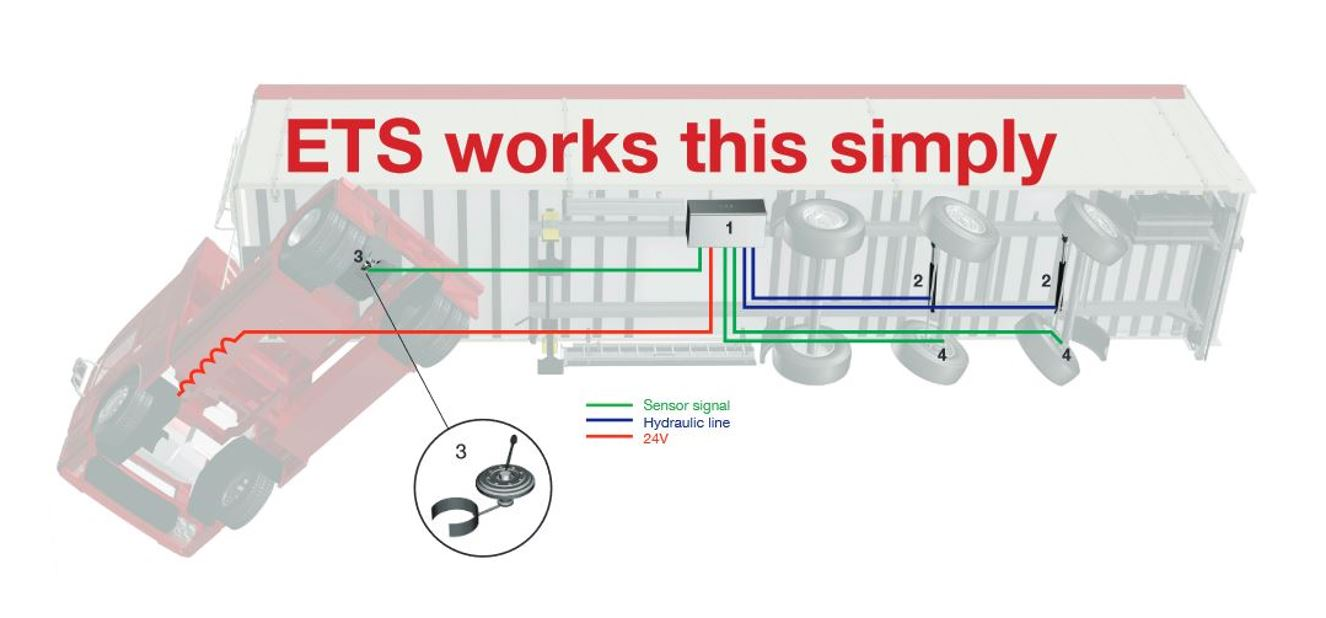
\includegraphics[width=1.0\linewidth]{figures/legacy_system_vse}
\caption[]{Active dolly legacy steering system supplied by VSE\cite{dolly_datasheet}}
\label{fig:legacy_system_vse}
\end{figure}





Short overview for the dolly, including: 

\begin{itemize}
\item mechanical properties in short (weight, turning radius, max. tonnage)
\item description of function (brake, steer, countersteer, lock at highspeed)
\item difference low $<=>$ high speed
\item control system by VSE, diagnosis, display connection with truck
\item system overview picture/schematics
\end{itemize}
\section{Real-Time Environment}
\label{sec:realtime_environment}



\begin{itemize}
	\item mechanical properties of box  (dimension, currents, mounting points in dolly)
	\item computational power/limitations
	\item explain interfaces with truck/dolly (abstract)
	\item explain technical realisation of HW interface (ZIF)
	\item explain rapid-prototyping
	\item robustness
	\item programming with software ref to \ref{sec:matlab}
	\item runtime interface ref to \ref{sec:control_desk}
\end{itemize}

\section{Interfaces with dolly}
\label{sec:interface_with_dolly}

\begin{itemize}
	\item private CANbus with AngleSensor for kingpin
	\item Vehicle CAN (ISO 11992, connector ISO 7638-2)
	\subitem brake by-wire
	\subitem EBS, ABS
	\subitem sensors for EBS, ABS
	\subitem signals/msgs on vehCAN
	\item physial interface =$>$ diagnosis outlet
\end{itemize}

\section{Interfaces with truck}
\label{sec:interface_with_dolly}

\begin{itemize}
	\item CAN communication with truck
	\item steering system conncetion

\end{itemize}


\section{Measurment Setup}
\label{sec:measurement_setup}

\subsection{On-board sensors}
\begin{itemize}
	\item king pin angle
	\subitem mounting
	\subitem CANcomm
	
	\item steering angle 
	\item speed
\end{itemize}


\subsection{Inertial measurement unit}
\label{sec:IMU}
To determine the processing delays in the control chain (refer to chapter \ref{chap:processing_time_delay}) as well as logging implementation for verification and analyses purposes a number of inertial measurement units (IMU) where utilizied throughout this thesis' work. The system at hand combined a gyroscope (L3GD20H), and an accelero- and magnetometer (LSM303D) into an IMU put on one circuit board.\cite{IMU_homepage_shop} This one-chip solution allowed for a convenient access to the sensor measurings, as the sensor outputs could be received via Inter-Integrated Circuit-protocol (I$^{2}$C)  which eliminates the need for transducer. Furthermore a high-pass filter is integrated into the IMU's accelerometer, which allows for easier compensation of the immanent drift. 

These units supply the measurings for three axes each at a maximum frequency of 1600Hz for the accelerometer and 757.6Hz for the gyroscope. \cite{accelerometer_datasheet}\cite{gyrometer_datasheet}


\subsection{Arduino Due}
\label{sec:arduino}

To parse the IMU's sensor output (see also section \ref{sec:IMU}) and convert it into a measurable format, it was decided to rely on the cost-efficient and robust Arduino platform. The Arduino platform was developed by  SmartProjects company in Italy and consists of a micro-controller board with several in- and output pins and a set of programming tools to program said micro-controller. This platform allows for a farely easy programming of the micro-controller in C with the help of some standard-libraries that make accessing the microcontroller's analog and digital in- and outputs very convenient. Additionally the downloading process to the micro-controller is simplyfied by a special boot-loader incorporated on the platform eliminating the need for special microcontroller programmers. 

SmartProjects offers various Arduino boards mainly differing in number of communication pins, memory size, clock frequency and physical size. It was decided to utilize the most powerful Arduino Due, offering 84 MHz of clock-speed, 512kB flash memory for programm-code and a 96kB working SRAM. This was done in order to allow for future use of this platform in other projects and having enough space for different sub-programs on the controller as well as enough processing power to deal with basic signal filtering and parsing at appropriate speeds. The Due also has a native I$^{2}$C interface, which was used to gather the measurings from the IMU. In addition the Due offers an abundance of 54 digital and 12 analog I/O-pins. Most importantly it comes with an on-board CAN-controller for measurement transfer to the logging system, eliminating the need for additional hardware for CAN-bus interfacing or bitbanging the CAN-communication. Furthermore the price-difference between the Due and smaller models is marginal. 

Besides the power-supply and the IMU-chip a MCP2551 CAN-transceiver by Microchip Technology Inc. was incorporated to take care of the pyhsical layer of CAN-bus communication by converting the digital signals from the Due's CAN-controller to the standardized voltage levels of the CAN. The MCP2551 is capable of different CAN standards and fully ISO-11898 compatible, which makes future use in different environments or as unit for in-vehicle CAN-interfacing feasible.


\begin{itemize}
	%\item clock frequency
	%\item RAM/ROM
	%\item ISP flash
	%\item robustness, reliability, cost-effectiveness
	\item input/outputs analog $\&$ digital
	\item native I2C capability
	\item CANcomm except of physical layer/transceiver available (OSI reference!) --$>$ no bit-banging needed --$>$ faster
\end{itemize}





\end{document}
